% !TeX program = lualatex
% !TeX root = main.tex
\renewcommand*{\dictumwidth}{0.7\textwidth}
\setchapterpreamble[u]{%
	\dictum[Gordon E. Moore%\footnotemark
]{``The complexity for minimum component costs has increased at a rate of roughly a factor of two per year... Certainly over the short term this rate can be expected to continue, if not to increase. Over the longer term, the rate of increase is a bit more uncertain, although there is no reason to believe it will not remain nearly constant for at least 10 years. That means by 1975, the number of components per integrated circuit for minimum cost will be 65,000. I believe that such a large circuit can be built on a single wafer.''}}

\chapter{Modelling the Processor Power Consumption}
\label{chap:model}
\bigskip
\textit{A formula describing the power consumption of a processor using its voltage and frequency, as well as different approximations about how to calculate this consumption based on reference values will be formulated and compared in this chapter.}
%\footnotetext{\url{ftp://download.intel.com/museum/Moores_Law/Articles-Press_Releases/Gordon_Moore_1965_Article.pdf}}

\bigskip
\lettrine[lines=2, lhang=.1, lraise=.1]{A}{s} seen in the previous chapter, the cluster energy consumption depends heavily on the used CPUs. The power consumption of a CPU ($P_{total}$) consists of a dynamic ($P_{dyn}$), a leakage ($P_{leak}$) and a short circuit power consumption ($P_{short}$). Additionally, recent processors include more and more components being formerly part of the mainboard. Those components are separated from the cores and are called ``uncore''. The main reasons for this are latency reduction (integration of the memory-controller), power efficiency (separate power control unit) and better scalability with many cores. Depending on processor type, uncore includes e.\,g. the memory-controller, L3 cache or PCIE-links. Of course the power consumption depends on the number of cores, too.
%
\begin{align}
P_{total} &= \#cores \cdot ( P_{dyn} + P_{leak} + P_{short} ) + uncore\nonumber
\end{align}
%
The uncore part of the chip drains between 4\,W and 20\,W. There is by now no generic formula to calculate the power consumption of the uncore-part, and measurement can only be done with special equipment\cite{ht4uCPU}. For these reasons, uncore is considered to be constant and added to the mainboard power consumption.\\[4em]
%
Back to the main components of $P_{total}$:
%
\begin{description}
	\item[$P_{short}$] is the power caused by a short-circuit current which flows from the supply to ground during a transition period of input signals when transistors are momentarily on at the same time. Short-circuit current increases with slower signal transition times\cite{HOT96}.

``The short circuit power consumption occurs only during signal transitions and is negligible''\,\cite{martin}.

	\item[$P_{leak}$] is the gradual loss of energy from charged capacitors or when current leaks out of the intended circuit. $P_{leak}$ is modelled differently depending on the actual research and application \cite{martin, power, temp}. It is possible that leakage power drains up to 20\,\% of $P_{total}$. So, further model improvements could include $P_{leak}$, because of its temperature dependency: $ P_{leak}\,\propto \, T^2 \cdot V$ \cite{tempaware}.
	\item[$P_{dyn}$] is the power used to actually charge and discharge the capacitance, composed of gate and interconnect capacitance.
%
The greater this dynamic switching current is, the faster capacitive loads can be charged and discharged, enabling a better performing circuit.
\end{description}

\noindent
Nowadays $P_{dyn}$ dominates\cite{power} and modelling the processor power consumption can be done with 
\begin{itemize}
	\item $U$, the supply voltage (often referred as $CPU$ $V\kern-0.3em core$ or $V_{DD}$) [V],
	\item $f$, the frequency the processor runs at [Hz]
\end{itemize}
and
\begin{itemize}
	\item $\alpha$, an activity factor (not all gates are always switched),
	\item $C$, the capacitance at the gate outputs [F].
\end{itemize}
%
So actually, $P_{short}$ and $P_{leak}$ will be ignored and only $P_{dyn}$ considered, 
%
\begin{align}
O(P_{dyn}) &\in O(P_{dyn} + P_{leak} + P_{short}). \nonumber
\end{align}
%
Which leads to an accurate estimation of the power consumption a processor core is using\,\cite{minartz}:
%
\begin{align}
P_{core} &\approx P_{dyn}\nonumber\\
&= U^2 \cdot f \cdot \alpha \cdot C\label{eq:main}
\end{align}
%
$U$ is the dominating factor, which means power consumption reduces linear by decreasing the frequency, whereas decreasing the voltage reduces the power consumption quadratically.

By writing about ``processor power consumption'' in this thesis, it is always meant per core and without uncore.

%
%
\section{Voltage²-frequency}
The factors $\alpha$ and $C$ from the previously introduced power consumption formula\,\eqref{eq:main} are depending on many different influences like processor type, workload or temperature. To avoid measuring\,/\,guessing $C$ and $\alpha$, they are considered constant at equal workloads on a given processor:
%
\begin{align}
const &= \alpha \cdot C \nonumber \\
\Rightarrow P &= U^2 \cdot f \cdot const \nonumber \\
%
\intertext{%
Having measured two (or more) power consumptions $P_{1}$ and $P_{2}$ at different voltages ($U_1$, $U_2$) respectively frequencies ($f_1$, $f_2$) of a processor results in an easy transformation equation:}
%
\label{eq:V2f}
const &= \frac{P}{U^2 \cdot f} \nonumber \\
\Rightarrow P_{2} &= P_{1} \cdot \frac{U^2_2}{U^2_1} \cdot \frac{f_2}{f_1}
\end{align}
%
The estimated power consumption of a processor $P_{2}$ can be calculated by having a reference value triple $P_{1}$, $U_1$ and $f_1$, and the new voltage $U_2$ and frequency $f_2$, without having to deal with the actual activity $\alpha$ respectively capacitance $C$.

\section{Approximations}
\label{sec:approximations}
%\todo{ähnlich einleiten bei den subs}
Sometimes there is no possibility to measure the voltage. Either the mainboard has no interfaces for software, only \lstinline!root! can use them or there is no adequate software installed\,/\,available.

In the following subsections are approximations described dealing without or only partial\,/\,general information about the supply voltages.

\subsection{Frequency³ Approach}
\label{sec:freq3}
If no access to any voltages is available, a simplifying approach is to assume, that changing the voltage also requires to change the frequency at the same amount. Generally speaking $f_{max}$ $\propto$ $U$. This leads to $U = \beta \cdot f$, where $\beta$ is another constant\,\cite{efficientserverclusters}.
%
\begin{align}
	P &= U^2 \cdot f \cdot const \nonumber \\
	U &= \beta \cdot f \label{eq:ubetaf} \\
	\nonumber \\
	\Rightarrow P &= f^3 \cdot const \nonumber \\
	\Rightarrow P_{2} &= P_{1} \cdot \frac{f^3_2}{f^3_1}\label{eq:f3}
\end{align}
%
In contrast to equation\,\eqref{eq:V2f}, the power consumption consists only of the former and the recent frequencies ($f_1$ and $f_2$).

\subsection{Extending Approximation}
\label{sec:approx}
The connection between the voltage, the frequency and the actual power consumption is unfortunately a bit more complicated, especially at lower voltages. From \cite{power} it is known, that 
\begin{align*}
f_{max} \, \propto \, \frac{(U_{supply} - U_{threshold})^2}{U_{supply}},
\end{align*}
where $U_{supply}$ is the supply voltage and $U_{threshold}$ the threshold voltage.
The threshold voltage at the gate is needed to prevent the creation of current from the drain to the source of the transistor. If $U_{supply}$ is bigger than $U_{threshold}$ the transistor is on, and vice versa. 

In order to lower $U_{supply}$, there is a constraint to reduce $U_{threshold}$ too. But a reduction of $U_{threshold}$ means, that $P_{leak}$ (and therefore $P_{core}$) rises, because of $P_{leak} = I_{leak} \cdot U_{supply}$ and the proportionality $I_{leak} \propto \exp(−U_{threshold} \cdot \frac{q}{kT})$\cite{vt}.

While this knowledge does not help to improve the approximation directly, it does help focusing on the problems.
%
\begin{figure}[h]
	\centering
	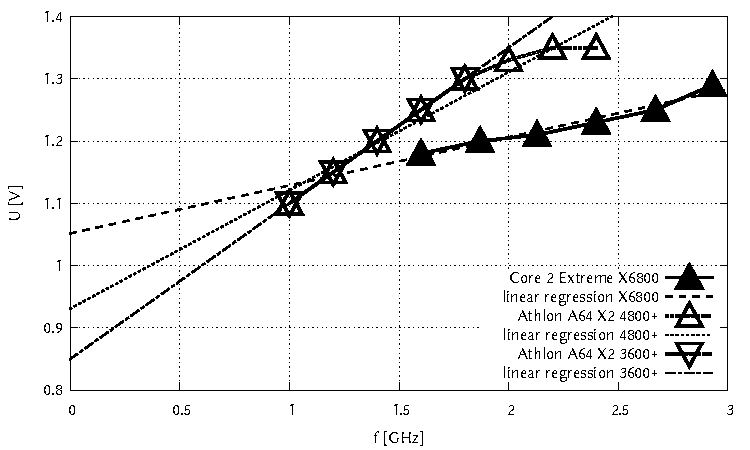
\includegraphics[width=\linewidth]{pix/pstates/pstates}
	\caption{P-state trend lines}
	\label{fig:pstates}
\end{figure}

%\noindent
In picture \ref{fig:pstates} are some valid $f$\,/\,$U$-pairs from more or less recent CPUs and a linear regression line for each.
It seems that $U$ and $f$ actually are in a linear relationship. But they are not proportional towards each other. The equation should rather be $U = \beta \cdot f + \gamma$, whereas $\beta$ is the gradient and $\gamma$ the y-intercept. Replacing $U$ results in
%
\begin{align}
	P &= U^2 \cdot f \cdot const \nonumber \\
	U &= \beta \cdot f + \gamma \label{eq:Ubetagamma}\\
	\nonumber \\
	\Rightarrow P &= (\beta \cdot f + \gamma)^2 \cdot f \cdot const \nonumber \\
	\Rightarrow P_{2} &= P_{1} \cdot \frac{f_2}{f_1} \cdot \frac{(\beta \cdot f_2 + \gamma)^2}{(\beta \cdot f_1 + \gamma)^2}
\end{align}
%
It can be seen in figure\,\ref{fig:pstates} that $\beta$ and $\gamma$ are different for every processor type. In order to calculate them, there has to be at least two valid $f$\,/\,$U$-pairs. Equation\,\eqref{eq:Ubetagamma} results directly in
%
\begin{align}
	\Rightarrow \beta &= \frac{\Delta U}{\Delta f} \qquad\text{and}\\
	\Rightarrow \gamma &= U_1 - f_1 \cdot \frac{\Delta U}{\Delta f}
\end{align}
%
By having introduced two new constants $\beta$ and $\gamma$ in equation\,\eqref{sec:freq3}, there is the option to eliminate one of them. 

Maybe it is easier to think about a y-intercept\,[$U$] than a gradient\,[$\frac{U}{f}$], but the actual choice depends, as always, on the use case.

\subsection{Intercept $\gamma$ Approach}
\label{sec:intercept}
Disappearing of $\beta$ starts again from equation\,\eqref{eq:Ubetagamma}:
%
\begin{align}
	\frac{U - \gamma}{f} &= \beta \nonumber \\
	\frac{U_1 - \gamma}{f_1} &= \frac{U_2 - \gamma}{f_2} \nonumber \\
	\Rightarrow U_2 &= U_1 \cdot \frac{f_2}{f_1} + \gamma \cdot (1 - \frac{f_2}{f_1})\label{eq:intercept}
\intertext{Inserting $U_2$ in the main equation\,\eqref{eq:V2f} results in}
	P_{2} &= P_{1} \cdot \frac{(U_1 \cdot \frac{f_2}{f_1} + \gamma \cdot (1 - \frac{f_2}{f_1}))^2}{U^2_1} \cdot \frac{f_2}{f_1} \nonumber \\
	&= P_{1} \cdot \frac{(U_1 + \gamma \cdot (\frac{f_1}{f_2} - 1))^2}{U^2_1} \cdot \frac{f_2^3}{f_1^3}
\end{align}
%
In contrast to equation\,\eqref{eq:f3} there is now an additional factor involved, which is greater 1 when $f_1 > f_2$ and lesser 1 when $f_1 < f_2$---in contrast to approach\,\ref{sec:freq3} more power drainage by switching to lower speeds, less by higher speeds. It becomes $1$ by equality of $f_1$ and $f_2$ resulting in $P_1=P_2$. 

\subsection{Gradient $\beta$ Approach}
Analogue to subsection\,\ref{sec:intercept}, $\gamma$ will vanish and the result becomes part of the main equation\,\eqref{eq:V2f}.
%
\begin{align}
	U - \beta \cdot f &= \gamma \nonumber \\
	U_1 - \beta \cdot f_1 &= U_2 - \beta \cdot f_2 \nonumber \\
	\Rightarrow U_2 &= U_1 - \beta \cdot (f_1 - f_2) \label{eq:gradient} \\
\nonumber \\
	P_{2} &= P_{1} \cdot \frac{(U_1 - \beta \cdot (f_1 - f_2))^2}{U^2_1} \cdot \frac{f_2}{f_1}
\intertext{In order to stay consistent with the equations of the other approximations, altering above equation for sake of simplicity produces:}
	P_{2} &= P_{1} \cdot \frac{(U_1 \cdot \frac{f_1}{f_2} - \beta \cdot (\frac{f_1^2}{f_2} - f_1))^2}{U^2_1} \cdot \frac{f_2^3}{f_1^3} \nonumber
\end{align}
%
but equation\,\eqref{eq:gradient} should rather be used for real-world application.

\superpar
As seen, the two extended approximations from section\,\ref{sec:approx} both need $U_1$ and the gradient $\beta$ or the intercept $\gamma$, in addition to $f_1$ and $f_2$. Nevertheless, there is no reason to use the first approximation from section\,\ref{sec:freq3}. $U_1$ can be seen in the BIOS (basic input output system) while booting, or asking the admin\,/\,support for its value. For $\beta$ or $\gamma$ some average values could be used. This should deliver acceptable results, as a short comparison shows.
\label{sec:summary}
%
\begin{figure}[!hb]
	\centering
	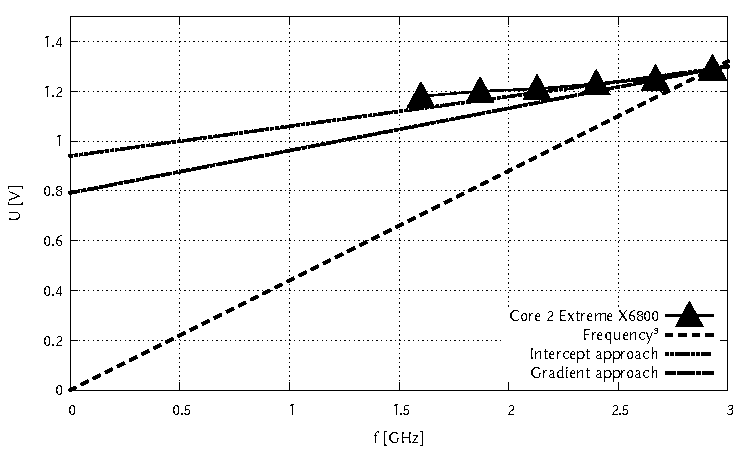
\includegraphics[width=\linewidth]{pix/modelcompare/modelcompare}
	\caption[Comparison between the approximations]{Comparison between the approximations ($\beta = 0.17$, $\gamma = 0.94$)}
	\label{fig:modelcompare}
\end{figure}
%

\noindent
Figure \ref{fig:modelcompare} shows a comparison between the three approximations discussed above at an example processor (taken from table \ref{tbl:approximations}), mean values for $\beta = 0.17$ and $\gamma = 0.94$ and the following derived formulas:

%
\begin{align*}
\text{Frequency³ approach \eqref{eq:ubetaf}} &\Rightarrow U_2 = U_1 \cdot \frac{f_2}{f_1}\\
\text{Intercept approach \eqref{eq:intercept}} &\Rightarrow U_2 = U_1 \cdot \frac{f_2}{f_1} + \gamma \cdot (1 - \frac{f_2}{f_1})\\
\text{Gradient approach \eqref{eq:gradient}} &\Rightarrow U_2 = U_1 - \beta \cdot (f_1 - f_2)\\
\end{align*}
%
It is obvious that the frequency³ approach is not able to compete against the other two. The assumption $f \, \propto \, V$ can not be considered at lower frequencies, resulting in too low estimated power consumptions.


%\newpage
%
%
\section{Power Saving Techniques}
As pointed out in this chapter, processors need much energy when calculating, and there is a great potential of reducing the power consumption of them. Power saving is implemented in hardware and in software, as those two have to work closely together in order to save the most energy without performance degradation.

%
\begin{description}
\item[Dynamic Voltage and Frequency Scaling] is the direct consequence from this chapter and possibly the most known technique. Based on its utilization the processor decreases its frequency and voltage in order to decrease power consumption too---the processor should only be as fast as needed, and therefore use as low power as possibly.\label{item:dvfs}

Mobile devices like notebooks or smart-phones use DVFS already a long time, since they notably rely on low energy consumption. Nowadays, DVFS is widespread among desktop PCs and server, and latterly some HPC cluster are using it too.

%
\begin{figure}[hbt]
	\centering
	\newcommand*\Captiontext{DVFS in multicore-processors}
	%\hfill %
		\subfloat[DualCore shared Freq \& Vcore]{% !TeX program = lualatex
% !TeX root = ../../main.tex
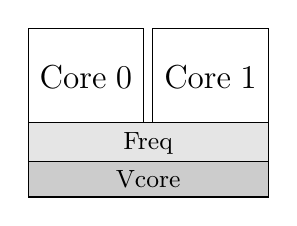
\begin{tikzpicture}[every node/.style={text centered}]
		\draw (0em, 0em)		node[rectangle, draw, text width=3.5em, minimum height=3.5em]
				{\large{Core 0}}
			(4.5em, 0em)	node[rectangle, draw, text width=3.5em, minimum height=3.5em]
				{\large{Core 1}}

			
			(2.25em, -2.4em)	node[rectangle, draw, text width=8em, minimum height=1.3em, fill=gray!20]
				{\small{Freq}}
			(2.25em, -3.7em)	node[rectangle, draw, text width=8em, minimum height=1.3em, fill=gray!40]
				{\small{Vcore}}
;
\end{tikzpicture}}
	\hfill % alternativ auch \hspace{1cm} für genaue Angaben
		\subfloat[QuadCore half-split Freq, shared Vcore]{% !TeX program = lualatex
% !TeX root = ../../main.tex
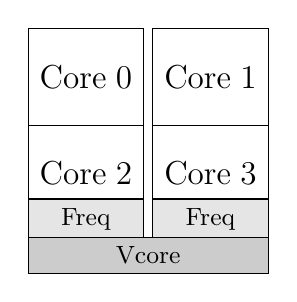
\begin{tikzpicture}[every node/.style={text centered}]
	\draw 	(0, -1.5em)		node[rectangle, draw, text width=3.5em, minimum height=3.5em]
				{\large{Core 0}}

			(4.5em, -1.5em)		node[rectangle, draw, text width=3.5em, minimum height=3.5em]
				{\large{Core 1}}

			(0, -5em)		node[rectangle, draw, text width=3.5em, minimum height=3.5em]
				{\large{Core 2}}
			(0, -6.65em)	node[rectangle, draw, text width=3.5em, minimum height=1.3em, fill=gray!20]
				{\small{Freq}}

			(4.5em, -5em)		node[rectangle, draw, text width=3.5em, minimum height=3.5em]
				{\large{Core 3}}
			(4.5em, -6.65em)	node[rectangle, draw, text width=3.5em, minimum height=1.3em, fill=gray!20]
				{\small{Freq}}
			(2.25em, -7.95em)	node[rectangle, draw, text width=8em, minimum height=1.3em, fill=gray!40]
				{\small{Vcore}}
;
\end{tikzpicture}}
	\hfill % alternativ auch \hspace{1cm} für genaue Angaben
		\subfloat[QuadCore split Freq \& Vcore]{% !TeX program = lualatex
% !TeX root = ../../main.tex
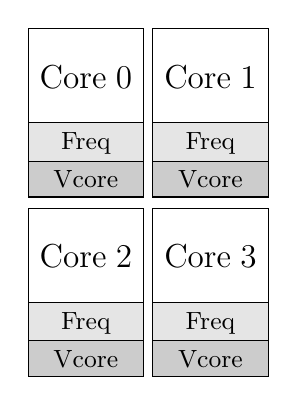
\begin{tikzpicture}[every node/.style={text centered}]
	\draw 	(0, 0)		node[rectangle, draw, text width=3.5em, minimum height=3.5em]
				{\large{Core 0}}
			(0, -2.4em)	node[rectangle, draw, text width=3.5em, minimum height=1.3em, fill=gray!20] 
				{\small{Freq}}
			(0, -3.7em)	node[rectangle, draw, text width=3.5em, minimum height=1.3em, fill=gray!40] 
				{\small{Vcore}}

			(4.5em, 0)		node[rectangle, draw, text width=3.5em, minimum height=3.5em]
				{\large{Core 1}}
			(4.5em, -2.4em)	node[rectangle, draw, text width=3.5em, minimum height=1.3em, fill=gray!20]
				{\small{Freq}}
			(4.5em, -3.7em)	node[rectangle, draw, text width=3.5em, minimum height=1.3em, fill=gray!40]
				{\small{Vcore}}

			(0, -6.5em)		node[rectangle, draw, text width=3.5em, minimum height=3.5em]
				{\large{Core 2}}
			(0, -8.9em)	node[rectangle, draw, text width=3.5em, minimum height=1.3em, fill=gray!20]
				{\small{Freq}}
			(0, -10.2em)	node[rectangle, draw, text width=3.5em, minimum height=1.3em, fill=gray!40]
				{\small{Vcore}}

			(4.5em, -6.5em)		node[rectangle, draw, text width=3.5em, minimum height=3.5em]
				{\large{Core 3}}
			(4.5em, -8.9em)	node[rectangle, draw, text width=3.5em, minimum height=1.3em, fill=gray!20]
				{\small{Freq}}
			(4.5em, -10.2em)	node[rectangle, draw, text width=3.5em, minimum height=1.3em, fill=gray!40]
				{\small{Vcore}}
;
\end{tikzpicture}}
	%\hfill %
	\caption[\Captiontext]{\Captiontext}
	\label{fig:dvfs}
\end{figure}
%

But DVFS has some disadvantages. 
\begin{itemize}
\item It only reduces $P_{dyn}$, but $P_{leak}$ will grow strongly in the future\cite{temp} due to further miniaturization.
\item As shown in figure \ref{fig:dvfs}, voltage and frequency can not always be free chosen. This is heavily processor and architecture dependent.
\item It takes time (and energy) to switch to another frequency-\,/\,voltage-level. Wrong decisions in switching can either harm performance respectively power saving, and there is still no ``crystal ball'' available.
\end{itemize}

\item[``Sleeping''] is used when a core has no work to do. This is done by deactivating parts of the core (ALUs, caches) or the complete core itself via clock-\,/\,power-gating, meaning to lower or even cut the frequency or the voltage. There exist different sleep states; the ``deeper'' the sleep the less power is consumed, but the longer it takes to wake up. A core can not execute instructions while sleeping.
\label{item:sleeping}

The disadvantages are mainly the same as for DVFS\cite{anand}.

\item[Idle-aware Scheduling] describes the idea of scheduling the processes in such a way, that many cores can sleep deeply.
This has to be done by the OS in order to gain the most of DVFS and sleeping.

This can of course mean some performance loss as processes have to use the same resources on a core. The opposite idea is to spread the processes on many cores for more performance and faster responses, but higher power consumption\cite{scheduler}.

\item[Intel Turbo Boost\,/\,AMD Turbo Core] Both Intel and AMD have implemented automatic overclocking features into their newer CPUs increasing their maximum frequency when the thermal budget is not yet reached. This is mainly the case, when single-threaded applications only stress individual cores. In this case, the other cores can sleep---their thermal budget is unused.
It is controversial calling dynamic overclocking a power saving technique, because the power consumption increases disproportionate to the performance gain.

Nevertheless it could help reducing the power consumption, because the faster some work is done, the longer the cores can sleep. The OS is also able to schedule processes longer on less cores when they ran faster, affecting again the sleep time of the remaining cores.

Turbo Boost\,/\,Turbo Core is all done hardware-side and transparent to the OS. By now, the only possibility for the OS\,/\,user to check if Turbo Boost\,/\,Turbo Core is in use is counting the CPU-cycles\cite{turboboost}.
\end{description}